\section{Evaluation}
\label{sec:experi}
We evaluate two system questions: how efficiently JHQ's primary representation
can be executed on a GPU, and how refinement demand varies across workloads.
We then measure recall--throughput operating regions, calibration and held-out
risk, controlled execution ablations, CPU/GPU budget sensitivity, and
construction and memory costs.

\subsection{Setup and protocol}
\label{sec:setup}
Measurements use an RTX 5090 (32\,GB, 170 SMs), a Xeon Platinum 8470Q host
(208 logical CPUs), CUDA 13.0, driver 595.71.05, and cuVS 26.08.01.
Table~\ref{tab:data} lists the six datasets and routing configurations. OpenAI
uses DBpedia embeddings, BGE Italian Wikipedia, and Stella TREC24 BioGen. For
these datasets, preprocessing removes non-finite vectors, normalises nonzero
vectors, and holds out queries with seed 42; Stella queries are corpus
samples. All systems use the same exported vectors and squared-L2 top-10
ground truth.

\begin{table}[bp]
\centering
\caption{Database shape and JHQ routing; $n_q$ is the actual query count.}
\label{tab:data}
\footnotesize
\begin{tabular}{lrrrr}\toprule
Dataset & $N$ & $d$ & $n_q$ & $\mathit{nlist}$\\\midrule
vogue-768~\cite{data_vogue} & 932,328 & 768 & 1,000 & 4,096\\
arxiv-768~\cite{data_arxiv} & 2,253,000 & 768 & 1,000 & 8,192\\
bge-m3~\cite{data_bge} & 10,091,524 & 1,024 & 1,000 & 32,768\\
stella-trec24~\cite{data_stella} & 17,776,615 & 1,024 & 999 & 32,768\\
openai3-1536~\cite{data_openai1536} & 999,000 & 1,536 & 1,000 & 8,192\\
openai3-3072~\cite{data_openai3072} & 999,000 & 3,072 & 1,000 & 8,192\\\bottomrule
\end{tabular}
\end{table}

Frontier timing covers host query input to host result output for the entire
query set, averaging three warmed runs and excluding calibration. Three cold
Vogue builds yield recall 0.9852, 0.9842, and 0.9849; cross-build differences
below approximately $10^{-3}$ therefore require repeated evidence. Small
timing differences are treated cautiously rather than as decisive
improvements.

JHQ uses $M=d/8$, $B=B_r=8$, 39 training points per centroid, eight coarse
iterations, and 100,000 residual-training vectors. Frontiers sweep
$\mathrm{nprobe}\in\{8,32,128,256,512,1024\}$. The primary system comparison
fixes $\alpha=100$, separating execution performance from budget selection.
The contextual calibrated curve uses $S=32$, $\epsilon=1$, and
$\alpha_{\max}=100$ on the evaluated pool. In a disjoint-half repetition, 18
of 36 selected budgets change although the mean selected-to-reference QPS
ratio remains similar, 1.60 versus 1.59. Similar aggregate speed ratios can
therefore hide different selected budgets, so calibration is evaluated
separately on held-out queries.

IVF-PQ sweeps eight-bit subcodes at 96--768-byte code lengths; CAGRA sweeps
graph degree, search width, and intermediate top-$k$. GPU memory is not
matched. Frontiers retain nondominated valid points, and matched-recall ratios
interpolate $\log$ QPS without extrapolation. Code and evaluation scripts will
be released upon publication.

\subsection{RQ1: End-to-end operating regions}
\label{sec:rq1}
Figure~\ref{fig:frontier} shows workload-dependent operating regions rather
than uniform dominance. CAGRA is 1.45--2.03$\times$ faster on the
768-dimensional datasets at recall 0.90/0.95. JHQ approaches parity on
OpenAI-1536 at 0.95 and reaches 1.52$\times$ CAGRA's QPS at 0.98; the
corresponding OpenAI-3072 ratios are 0.66 and 1.09. IVF-PQ is slower at the
evaluated targets within common measured coverage.

\begin{figure}[!htbp]
\centering
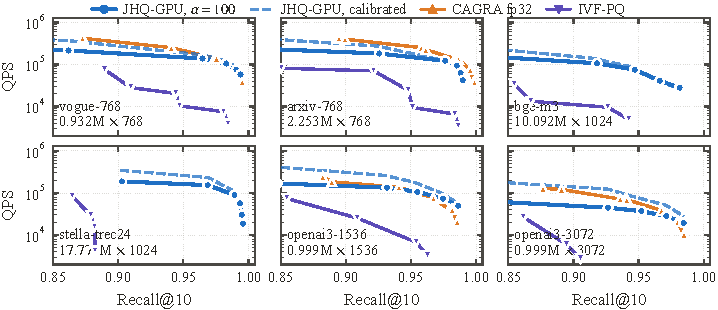
\includegraphics[width=\linewidth]{figs/fig_frontier.pdf}
\caption{Recall@10--QPS, entire query set per call. Solid JHQ fixes
$\alpha=100$; dashed calibrates on a 32-query sample of the evaluated pool and
excludes calibration cost, so it is contextual rather than held out.
Section~\ref{sec:rq2} evaluates calibration on held-out queries. Endpoints are
measured sweep endpoints.}
\label{fig:frontier}
\end{figure}

JHQ separates routing coverage from second-level work: increasing
$\mathrm{nprobe}$ visits more inverted lists, whereas $\alpha k$ bounds how
many screened candidates receive residual scoring. Broader routing can
therefore expand primary screening without requiring residual scoring of every
additional candidate. At $\alpha=100$ and $\mathrm{nprobe}=32$, residual
refinement accounts for approximately 57\% of measured work on Vogue and 70\%
on OpenAI-3072. Each retained candidate requires its residual code to be read
and scored, so a large fixed survivor set remains costly even when primary
screening is efficient. Reducing that set avoids residual work, but candidates
discarded during screening cannot be recovered later. Refinement is therefore
a substantial remaining cost in these measured cells, and the survivor budget
controls both the available acceleration and the risk of losing useful
neighbours.

For baseline fairness, IVF-PQ is reported under the better measured
partitioning between its own and JHQ's. CAGRA exceeds the device memory
capacity during construction on BGE and Stella, so the missing points mark a
feasibility boundary on this device rather than a search-quality failure. One
contaminated Stella measurement is excluded throughout.

\subsection{RQ2: Budget selection, quality, and calibration cost}
\label{sec:rq2}
\paragraph{Protocol and workload variation.}
Each dataset uses one shared index for fixed budgets, sampled calibration,
full-pool calibration, same-sample enumeration, and an offline oracle.
Even-indexed queries calibrate; odd-indexed queries evaluate. The grid is
$\{200,100,64,32,16,8,4,2\}$ with $\epsilon=1$. Across probes 128 and 512, the
oracle chooses the fastest grid point within $10^{-3}$ of the best measured
held-out recall. Its budgets range from 4 to 200, and the sampled rule's
median agrees in ten of twelve configurations at $S=128$
(Table~\ref{tab:budget}). This variation motivates workload-specific control
of $c_k=\alpha k$: a shared constant can spend refinement work where little is
gained or restrict it where additional candidates improve the result. Median
agreement alone does not establish quality for every calibration draw.

\begin{table}[bp]
\centering
\caption{Held-out budget comparison, $\epsilon=1$, $\alpha_{\max}=200$. Each
cell gives $\alpha$ and Recall@10, then kQPS. Rule entries are the median
$\alpha$, mean recall and mean selected-arm QPS over 64 draws at $S=128$.}
\label{tab:budget}
% Generated by figures/current_budget.py
\footnotesize\setlength{\tabcolsep}{3.5pt}
\begin{tabular}{@{}lccccc@{}}\toprule
Dataset / probe & Fixed 64 & Fixed 100 & Rule & Full pool & Oracle \\ \midrule
vogue\,/\,128 & \shortstack{$64;\ 0.9678$\\$143.2$} & \shortstack{$100;\ 0.9680$\\$118.7$} & \shortstack{$64;\ 0.9677$\\$143.4$} & \shortstack{$100;\ 0.9680$\\$118.7$} & \shortstack{$64;\ 0.9678$\\$143.2$} \\
arxiv\,/\,128 & \shortstack{$64;\ 0.9736$\\$155.4$} & \shortstack{$100;\ 0.9748$\\$114.0$} & \shortstack{$100;\ 0.9751$\\$100.0$} & \shortstack{$200;\ 0.9760$\\$66.4$} & \shortstack{$200;\ 0.9760$\\$66.4$} \\
openai3-1.5k\,/\,128 & \shortstack{$64;\ 0.9280$\\$146.6$} & \shortstack{$100;\ 0.9280$\\$124.4$} & \shortstack{$8;\ 0.9279$\\$248.5$} & \shortstack{$8;\ 0.9280$\\$248.9$} & \shortstack{$8;\ 0.9280$\\$248.9$} \\
openai3-3k\,/\,128 & \shortstack{$64;\ 0.9252$\\$81.5$} & \shortstack{$100;\ 0.9252$\\$42.4$} & \shortstack{$4;\ 0.9252$\\$117.5$} & \shortstack{$4;\ 0.9252$\\$117.5$} & \shortstack{$4;\ 0.9252$\\$117.5$} \\
bge\,/\,128 & \shortstack{$64;\ 0.9192$\\$110.0$} & \shortstack{$100;\ 0.9198$\\$100.0$} & \shortstack{$32;\ 0.9190$\\$120.3$} & \shortstack{$64;\ 0.9192$\\$110.0$} & \shortstack{$32;\ 0.9190$\\$124.8$} \\
stella\,/\,128 & \shortstack{$64;\ 0.9892$\\$91.9$} & \shortstack{$100;\ 0.9892$\\$84.8$} & \shortstack{$16;\ 0.9884$\\$103.3$} & \shortstack{$16;\ 0.9886$\\$103.1$} & \shortstack{$16;\ 0.9886$\\$103.1$} \\
vogue\,/\,512 & \shortstack{$64;\ 0.9914$\\$72.4$} & \shortstack{$100;\ 0.9914$\\$64.8$} & \shortstack{$64;\ 0.9913$\\$71.1$} & \shortstack{$100;\ 0.9914$\\$64.8$} & \shortstack{$64;\ 0.9914$\\$72.4$} \\
arxiv\,/\,512 & \shortstack{$64;\ 0.9844$\\$68.9$} & \shortstack{$100;\ 0.9878$\\$58.9$} & \shortstack{$200;\ 0.9885$\\$50.4$} & \shortstack{$200;\ 0.9894$\\$41.3$} & \shortstack{$200;\ 0.9894$\\$41.3$} \\
openai3-1.5k\,/\,512 & \shortstack{$64;\ 0.9740$\\$70.4$} & \shortstack{$100;\ 0.9740$\\$68.3$} & \shortstack{$8;\ 0.9738$\\$97.2$} & \shortstack{$8;\ 0.9740$\\$97.2$} & \shortstack{$8;\ 0.9740$\\$97.2$} \\
openai3-3k\,/\,512 & \shortstack{$64;\ 0.9704$\\$39.0$} & \shortstack{$100;\ 0.9704$\\$27.5$} & \shortstack{$4;\ 0.9702$\\$49.4$} & \shortstack{$4;\ 0.9702$\\$49.4$} & \shortstack{$8;\ 0.9704$\\$49.6$} \\
bge\,/\,512 & \shortstack{$64;\ 0.9664$\\$40.1$} & \shortstack{$100;\ 0.9670$\\$38.7$} & \shortstack{$64;\ 0.9661$\\$40.8$} & \shortstack{$64;\ 0.9664$\\$40.1$} & \shortstack{$64;\ 0.9664$\\$40.1$} \\
stella\,/\,512 & \shortstack{$64;\ 0.9954$\\$29.6$} & \shortstack{$100;\ 0.9954$\\$29.0$} & \shortstack{$16;\ 0.9945$\\$30.9$} & \shortstack{$16;\ 0.9948$\\$30.9$} & \shortstack{$16;\ 0.9948$\\$30.9$} \\
\bottomrule\end{tabular}

\end{table}

\paragraph{Output stability and held-out quality.}
Figure~\ref{fig:budget}(a) shows that 27--98\% of draws at $S=32$ lose more
than $10^{-3}$ held-out recall relative to the best tested budget; at $S=128$,
counts range from zero to 40 of 64. For BGE at probe 512, 24 of 64 draws
exceed the $10^{-3}$ threshold, while the mean held-out recall loss is
approximately 0.0009 and the 95th percentile is 0.0014. The agreement test
observes only sampled outputs: a budget sufficient for those queries may
discard useful candidates for unseen queries, and the reference output itself
is approximate. Output stability is therefore a label-free heuristic rather
than a ground-truth recall guarantee. Increasing $S$ also tightens the allowed
disagreement fraction because $\epsilon=1$ is fixed, so the observed change
combines broader sampling with a stricter criterion; zero failures in repeated
draws from fixed pools do not establish zero risk.

\begin{figure}[tbp]
\centering
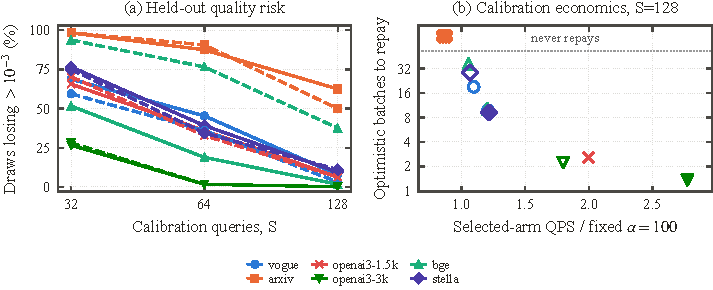
\includegraphics[width=\linewidth]{figs/fig_budget_current.pdf}
\caption{(a) Draws losing $>10^{-3}$ recall against the best tested budget;
solid/dashed lines denote probes 128/512. (b) Mean selected-arm QPS gain and
optimistic aggregate payback at $S=128$, relative to fixed $\alpha=100$;
filled/open markers denote probes 128/512. Payback uses 500-query equivalents.}
\label{fig:budget}
\end{figure}

\paragraph{Searching the budget grid.}
Bisection and enumeration agree in all 2,304 draws across $S\in\{32,64,128\}$;
enumeration costs 1.66--2.00$\times$ as much, including reference search.
Bisection saves work by testing only part of the grid, while the additional
tests in enumeration do not change the selected budgets on these samples. Thus
bisection makes the same sampled criterion cheaper; it does not remove the
criterion's held-out generalisation risk.

\paragraph{Benefit and reuse.}
At $S=128$, mean selected-arm QPS is 1.05--2.77$\times$ fixed-$\alpha=100$ QPS
in ten of twelve configurations. The arxiv configurations instead sacrifice
12--14\% throughput for higher mean recall because matching a larger reference
can require increasing the budget above the fixed comparison point.
Calibration costs 5.2--30.8\,ms, yielding an estimated payback of 1.4--36.4
batches of 500-query equivalents in configurations with throughput gains
(Figure~\ref{fig:budget}(b)). Calibration is paid once for a reusable budget,
whereas savings accumulate over subsequent batches; short workloads may end
before recovering this cost, and the slower arxiv selections never repay
through throughput. Selected-arm QPS averages previously measured fixed-arm
throughputs; taking the reciprocal of that average underestimates mean batch
time when selections differ, so the aggregate payback is optimistic.
Calibration includes reference search and agreement checks but excludes sample
gathering, and reuse assumes a stable workload.

\begin{table}[tbp]
\centering
\caption{Paired observations, each holding the represented distance fixed.
\emph{Cells} counts comparisons within a source experiment; the ranges do not
describe a common workload.}
\label{tab:neg}
\footnotesize
\begin{tabular}{ll@{\hspace{1.2em}}r@{\hspace{1.2em}}l}\toprule
Change & QPS effect & cells & Simple heuristic challenged\\\midrule
Table-free exact score & $-30$ to $-52\%$ & 12 & Minimum table state\\
$G=8$ versus $G=4$ & $-3.4$ to $-38.5\%$ & 24 & Equal footprint, equal speed\\
Packed 32-bit loads & $+1$ to $+66\%$ & 48 & Bytes moved predict speed\\
Private probe cursor & $-1.4$ to $+148.5\%$ & 20 & Loop work is negligible\\
\bottomrule
\end{tabular}
\end{table}

\subsection{RQ3: Which execution choices account for the gains?}
\label{sec:rq3}\label{sec:rq4}
The hierarchy ablation changes representation fidelity and is discussed
separately. The paired execution ablations in Table~\ref{tab:neg}, by
contrast, hold the represented distance fixed, allowing throughput differences
to be attributed to execution choices rather than to a different scoring
function.

\paragraph{Role of the hierarchy.}
Primary-only recall peaks at 0.5135--0.8642 across the six datasets, and
residual refinement extends every range. Residual codes supply information
omitted by the compact primary representation, improving the ranking among
retained candidates. Applying that additional precision only after screening
avoids residual scoring across the entire routed pool. Thus, $\alpha$ controls
how many candidates receive residual scoring, while residual-code precision
remains fixed. The ablation keeps the full allocation, so it does not measure
the memory of a minimal primary-only index.

\begin{figure}[bp]
\centering
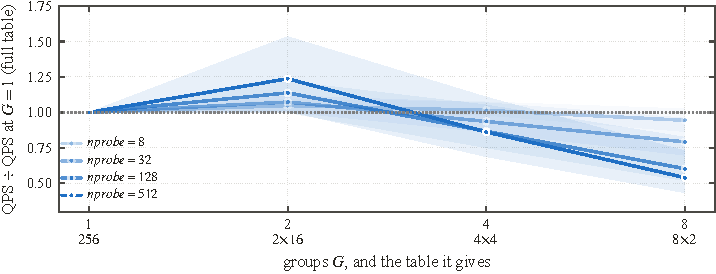
\includegraphics[width=0.78\linewidth]{figs/fig_lutgroups.pdf}
\caption{Throughput against the full table, six datasets at four probe
depths; lines are medians over datasets and bands their range. Factorising to
$G{=}2$ gains, factorising further gives it back, and both effects grow with
probe depth. $4{\times}4$ and $8{\times}2$ store the same 16 entries and
require different numbers of lookups.}
\label{fig:lutgroups}
\end{figure}

\paragraph{Table grouping.}
With represented distance fixed, $G=2$ leads in 23 of 24 configurations
(Figure~\ref{fig:lutgroups}); the exception favours $G=1$ by only 0.03\%.
Splitting 256 entries into two 16-entry tables reduces table state eightfold
with two lookups per candidate--subspace pair. Further splitting eventually
stops saving table state: $G=4$ and $G=8$ both store 16 entries per subspace,
but $G=8$ requires twice as many lookups and is observed to be 3.4--38.5\%
slower. The extra lookups recur throughout the scan without reducing table
footprint, showing why the smallest tables need not give the fastest search.

\paragraph{Packed access.}
Across 48 paired comparisons, packing improves QPS by 1--66\%, with a maximum
four-arm recall difference of 0.0001. A 32-bit load fetches four byte codes,
amortising address calculation and loop control across them while adding
register unpacking. The logical code volume and represented distance remain
unchanged, so the improvement is consistent with more efficient code access
rather than a different scoring approximation. Factorisation gains appear with
both byte and word loads, supporting their combination. All arms use
subspace-major storage, so transposition is not separately isolated;
differences near 1\% require stronger timing evidence.

\paragraph{Alternative execution choices.}
Table-free exact scoring is 30--52\% slower (Table~\ref{tab:neg}). Removing
tables replaces reusable query-specific distances with arithmetic repeated for
each candidate, while table construction occupies only 0.20--2.30\% of
measured batch time. Avoiding that small setup cost can therefore increase
work repeated throughout the scan. Changes to probe traversal likewise alter
throughput without changing logical code volume. These results show that
repeated execution work matters alongside storage, but they do not identify
instruction issue, cache behaviour, register pressure, or occupancy as the
dominant hardware bottleneck.

\subsection{RQ4: Does the CPU refinement budget transfer to the GPU?}
\label{sec:rq5}\label{sec:rq6cpu}
On OpenAI-3072, define the tuning gain as
\[
g=\frac{\mathrm{QPS}_{\mathrm{tuned}}}{\mathrm{QPS}_{100}}-1,
\]
where the tuned point is the fastest measured budget with at most 0.003 recall
loss relative to each implementation's own fixed-$\alpha=100$ result. Across
the shared probe depths 128--1024, $g_{\mathrm{GPU}}/g_{\mathrm{CPU}}$ is
2.5--3.0. Because reducing the survivor set removes residual work while
leaving routing and primary screening intact, the benefit of changing $\alpha$
depends on the relative stage costs. The larger relative tuning gain in the
measured GPU implementation therefore motivates retuning the inherited CPU
budget rather than carrying it over unchanged.

The comparison is a sensitivity result, not an identical-index hardware
speedup. The CPU uses 32 threads and separately trained codebooks, with 4,096
lists versus 8,192 on the OpenAI GPU frontiers. Probes below 128 are excluded
because thread start-up dominates, most CPU configurations are timed once, and
BGE and Stella have no CPU measurement. These differences limit attribution to
hardware alone.

\subsection{RQ5: Construction and memory costs}
\label{sec:rq6}
\begin{figure}[bp]
\centering
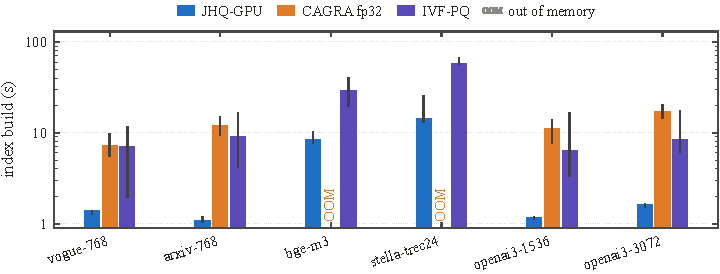
\includegraphics[width=\linewidth]{figs/fig_build.pdf}
\caption{Index build time, log scale. Bars are medians over clean
configurations and repeats, whiskers their range, not a confidence interval.
JHQ's bar is one cold training plus its median encode.}
\label{fig:build}
\end{figure}
In Figure~\ref{fig:build}, the fastest compared alternative per dataset takes
3.5--8.5$\times$ JHQ's estimated build time. Training contributes 71\% of
JHQ's estimate on Vogue but 27\% on Stella: training dominates the former,
while encoding dominates the latter. Both costs are paid before query-time
savings accumulate, making construction relevant to workloads that rebuild
frequently. Training budgets differ, including a reduced Stella IVF-PQ sample,
so the comparison reflects the measured configurations rather than a
controlled difference between quantisers.

\begin{figure}[!htbp]
\centering
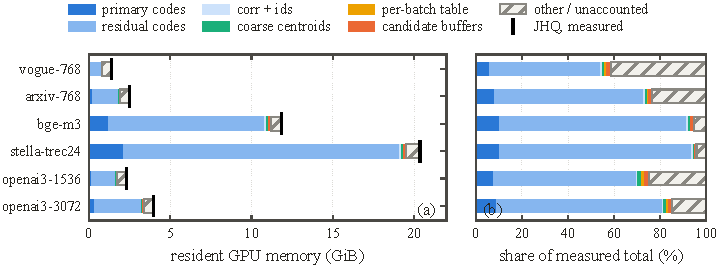
\includegraphics[width=\linewidth]{figs/fig_memory.pdf}
\caption{Resident memory by component: (a) absolute, markers at measured
totals; (b) the same stack as a share, where the five smaller sets are
readable. Hatched is the unattributed remainder.}
\label{fig:memory}
\end{figure}

Residual codes remain the largest memory component
(Figure~\ref{fig:memory}): 48\% of 1.4\,GiB on Vogue and 83\% of 20.4\,GiB on
Stella. Each vector retains eight residual bits per dimension alongside one
primary bit. A smaller survivor budget reduces how many residual codes are
read and scored per query but does not change their resident allocation; table
factorisation reduces query-specific table state rather than residual storage.
JHQ therefore trades resident residual capacity for selective query-time
compute, occupying a different memory--accuracy--throughput operating point
rather than being uniformly cheaper. The 4--41\% unattributed memory remainder
is reported separately.
